\def\year{2022}\relax
%File: formatting-instructions-latex-2022.tex
%release 2022.1
\documentclass[letterpaper]{article} % DO NOT CHANGE THIS
\usepackage{aaai22}  % DO NOT CHANGE THIS
\usepackage{times}  % DO NOT CHANGE THIS
\usepackage{helvet}  % DO NOT CHANGE THIS
\usepackage{courier}  % DO NOT CHANGE THIS
\usepackage[hyphens]{url}  % DO NOT CHANGE THIS
\usepackage{graphicx} % DO NOT CHANGE THIS
\urlstyle{rm} % DO NOT CHANGE THIS
\def\UrlFont{\rm}  % DO NOT CHANGE THIS
\usepackage{natbib}  % DO NOT CHANGE THIS AND DO NOT ADD ANY OPTIONS TO IT
\usepackage{caption} % DO NOT CHANGE THIS AND DO NOT ADD ANY OPTIONS TO IT
\DeclareCaptionStyle{ruled}{labelfont=normalfont,labelsep=colon,strut=off} % DO NOT CHANGE THIS
\frenchspacing  % DO NOT CHANGE THIS
\setlength{\pdfpagewidth}{8.5in}  % DO NOT CHANGE THIS
\setlength{\pdfpageheight}{11in}  % DO NOT CHANGE THIS
%
% These are recommended to typeset algorithms but not required. See the subsubsection on algorithms. Remove them if you don't have algorithms in your paper.
\usepackage{algorithm}
\usepackage{algpseudocode}
\usepackage{amssymb}
\usepackage{amsmath}
\usepackage{xcolor}
\usepackage{amsthm}
\usepackage{adjustbox}
\usepackage{multirow}

\usepackage{enumitem}
\newlist{myitemize}{itemize}{1}
\setlist[myitemize,1]{label=\textbullet,leftmargin=0pt}

% \newtheorem{theorem}{Theorem}
\newtheorem{definition}{Definition}
\newtheorem{theorem}{Theorem}[section]
\newtheorem{lemma}[theorem]{Lemma}
%
% These are are recommended to typeset listings but not required. See the subsubsection on listing. Remove this block if you don't have listings in your paper.
\usepackage{newfloat}
\usepackage{listings}
\lstset{%
	basicstyle={\footnotesize\ttfamily},% footnotesize acceptable for monospace
	numbers=left,numberstyle=\footnotesize,xleftmargin=2em,% show line numbers, remove this entire line if you don't want the numbers.
	aboveskip=0pt,belowskip=0pt,%
	showstringspaces=false,tabsize=2,breaklines=true}
\floatstyle{ruled}
\newfloat{listing}{tb}{lst}{}
\floatname{listing}{Listing} 
%
%\nocopyright

% PDF Info Is REQUIRED.
% For /Title, write your title in Mixed Case.
% Don't use accents or commands. Retain the parentheses.
% For /Author, add all authors within the parentheses,
% separated by commas. No accents, special characters
% or commands are allowed.
% Keep the /TemplateVersion tag as is
\pdfinfo{
/Title (Considering Theory of Mind in  Human-Aware Task Planning for a Collaborative Robot)
% /Author (Anthony Favier, Shashank Shekhar, Rachid Alami)
/Author Paper #8284)
/TemplateVersion (2022.1)
}

% DISALLOWED PACKAGES
% \usepackage{authblk} -- This package is specifically forbidden
% \usepackage{balance} -- This package is specifically forbidden
% \usepackage{color (if used in text)
% \usepackage{CJK} -- This package is specifically forbidden
% \usepackage{float} -- This package is specifically forbidden
% \usepackage{flushend} -- This package is specifically forbidden
% \usepackage{fontenc} -- This package is specifically forbidden
% \usepackage{fullpage} -- This package is specifically forbidden
% \usepackage{geometry} -- This package is specifically forbidden
% \usepackage{grffile} -- This package is specifically forbidden
% \usepackage{hyperref} -- This package is specifically forbidden
% \usepackage{navigator} -- This package is specifically forbidden
% (or any other package that embeds links such as navigator or hyperref)
% \indentfirst} -- This package is specifically forbidden
% \layout} -- This package is specifically forbidden
% \multicol} -- This package is specifically forbidden
% \nameref} -- This package is specifically forbidden
% \usepackage{savetrees} -- This package is specifically forbidden
% \usepackage{setspace} -- This package is specifically forbidden
% \usepackage{stfloats} -- This package is specifically forbidden
% \usepackage{tabu} -- This package is specifically forbidden
% \usepackage{titlesec} -- This package is specifically forbidden
% \usepackage{tocbibind} -- This package is specifically forbidden
% \usepackage{ulem} -- This package is specifically forbidden
% \usepackage{wrapfig} -- This package is specifically forbidden
% DISALLOWED COMMANDS
% \nocopyright -- Your paper will not be published if you use this command
% \addtolength -- This command may not be used
% \balance -- This command may not be used
% \baselinestretch -- Your paper will not be published if you use this command
% \clearpage -- No page breaks of any kind may be used for the final version of your paper
% \columnsep -- This command may not be used
% \newpage -- No page breaks of any kind may be used for the final version of your paper
% \pagebreak -- No page breaks of any kind may be used for the final version of your paperr
% \pagestyle -- This command may not be used
% \tiny -- This is not an acceptable font size.
% \vspace{- -- No negative value may be used in proximity of a caption, figure, table, section, subsection, subsubsection, or reference
% \vskip{- -- No negative value may be used to alter spacing above or below a caption, figure, table, section, subsection, subsubsection, or reference

\setcounter{secnumdepth}{0} %May be changed to 1 or 2 if section numbers are desired.

% The file aaai22.sty is the style file for AAAI Press
% proceedings, working notes, and technical reports.
%

% Title

% Your title must be in mixed case, not sentence case.
% That means all verbs (including short verbs like be, is, using,and go),
% nouns, adverbs, adjectives should be capitalized, including both words in hyphenated terms, while
% articles, conjunctions, and prepositions are lower case unless they
% directly follow a colon or long dash
\title
{
% old-1. Human-Aware Planning with Communication: \\ While Keeping Itself in Human's Shoes a Robot Plans for Both 
% Perspective Taking and Its Use for Communication in Planning: 
% Old Title 2:Planning with Communication Empowered by Situation Assessment:
% \\ 
% A Robot Builds Collaborative Plans
% while Keeping Itself in Human's Shoes
% Considering Theory of Mind in  Human-Aware Task Planning \\ for a Collaborative Robot
% Robust Task Planning for Human-Aware Collaborative Robots via Theory of Mind
Will They Know? Integrating Theory of Mind \\ in Human Aware Task Planning for Collaborative Robots
% Anticipating Human's Situation Assessment during \\ Robot Task Planning to Improve the Collaboration
% Robust Planning for Human-Robot Joint Tasks \\ with Explicit Reasoning on Human Mental State
%While Keeping Itself in Human's Shoes a Robot Produce Collaborative Plans 
%is in Human's Shoes   
% old-2. Towards a robot partner reducing\\ ambiguities using perspective taking
}
\author{
    %Authors
    % All authors must be in the same font size and format.
    % Anthony Favier\textsuperscript{\rm 1,2},
    % Shashank Shekhar\textsuperscript{\rm 1},
    % Rachid Alami\textsuperscript{\rm 1,2}
    Authors
}
\affiliations{
    % Afiliations
    % \textsuperscript{\rm 1}LAAS-CNRS, Universite de Toulouse, Toulouse, France\\
    % \textsuperscript{\rm 2}{Artificial and Natural Intelligence Toulouse Institute (ANITI)}

    % % email address must be in roman text type, not monospace or sans serif
    % \{anthony.favier, sshekhar, rachid.alami\}@laas.fr
    % Affiliations
}

\begin{document}

%%%%% SYMBOLS DEFINITION %%%%%
\newcommand{\worldstates}{\mathcal{S}}
\newcommand{\worldstate}{s}
\newcommand{\fluent}[3]{\mathcal{F}^{#1#2}_{#3}}
\newcommand{\prop}{\varphi}
\newcommand{\allprops}{\Phi}
\newcommand{\predicate}{\mathcal{P}}
\newcommand{\predval}{v}
\newcommand{\agent}{\lambda}
\newcommand{\beliefs}{\mathcal{B}}
\newcommand{\human}{H}
\newcommand{\robot}{R}
\newcommand{\places}{\mathcal{P}}
\newcommand{\place}{p}
\newcommand{\unknown}{UnKw}
\newcommand{\known}{Kw}
\newcommand{\missedactions}{\mathcal{M}}
\newcommand{\loc}[1]{loc(#1)}
\newcommand{\obs}[1]{obs(#1)}
\newcommand{\dom}[1]{dom(#1)}
\newcommand{\observable}{\texttt{OBS}}
\newcommand{\inferable}{\texttt{INF}}
%%%%%%%%%%%%%%%%%%%%%%%%%%%%%%

\maketitle

\begin{abstract}
% OLD
% Building on earlier work about human-aware planning and execution, we describe a new approach that:
% (a) models the robot’s capabilities to compute the spatial perspective of its human partner while following their activities; 
% and using that, (b) it estimates the evolution of the mental state of its human partner to perform robust planning for the human’s and robot’s joint tasks with a known objective to achieve.
% More specifically, our approach formalizes standard execution-time observability conventions based abstractly on situation assessment. Using this formalization during planning, it captures the evolution of human’s and robot’s beliefs to
% deal with belief divergences that could arise in practice and
% affect plan execution. While anticipating such a divergence, the approach decides \textit{if} and \textit{when} belief alignment is needed
% and achieves it using communication.  
% The proposed approach is sound and complete and generates robust plans for more realistic and challenging problems, and it uses communication effectively,
% i.e., without the robot giving unnecessary information that a collaborative human can observe or infer in practice.
% NEW

% anthony-v1
% When planning for a collaborative task, sharing the plan before execution is a common practice and assumption that may be verbally costly and even restrict the human's behavior. A recent approach named HATP/EHDA lifts this assumption and plans the robot actions while estimating the future human's behavior, without constraining it.
% For a proper interaction, Theory of Mind (ToM) must be considered by the robot. Several works integrate ToM at execution time to adapt online the robot's behavior to the human. However, such intelligent reactions may not always be enough. In some scenarios, ToM should be considered at planning time to be proactive. 
% Hence, we describe a new conceptual approach that: (a) plans the robot actions to achieve a joint shared goal with a human considered as uncontrollable,
% (b) manages the human's belief distinctly to predict their behavior and adapt the robot's one accordingly,
% (c) anticipates the upcoming spatial perspective of the human to better estimate their belief. 
% More specifically, we explain where and how Situation Assessment is inserted in the planning process. And we show, thanks to this addition, how ambiguous situations due to estimated false human beliefs can be detected and avoided by different means (communication or delay robot actions).  
% This conceptual approach has been implemented, and some qualitative and experimental results are discussed to show \textit{its potential}.

% anthony-v2
% Theory of Mind (ToM) must be considered by the robot to interact properly with humans. Several works integrate ToM at execution time to adapt online the robot's behavior to unplanned human initiatives. However, such online approaches may not always be enough and in some scenarios ToM should be considered during offline planning for the robot to be proactive. 
% On the other hand, when planning for a collaborative task, sharing the plan before execution is a common practice and assumption that has benefits but may be verbally costly and even restrict the human's behavior. Hence, adapting online the robot's behavior may involve replanning and sharing again the plan which can worsen the interaction quality.
% Recent offline planners provide more latitude to humans by discarding the idea of shared plan and considering the human as \textit{uncontrollable}. Indeed, they plan only for the robot's behavior while estimating future humans' behavior.
% Building on existing work, we describe a new offline planning approach that formalizes ToM to maintain agents' distinct beliefs 
% (a) plans the robot actions to achieve a joint shared goal with a human considered as uncontrollable,
% (b) manages the human's belief distinctly to predict their behavior and adapt the robot's one accordingly,
% (c) anticipates the upcoming spatial perspective of the human to better estimate their belief. 
% More specifically, we explain where and how Situation Assessment is inserted in the planning process. And we show, thanks to this addition, how ambiguous situations due to estimated false human beliefs can be detected and avoided by different means (communication or delay robot actions).  
% This conceptual approach has been implemented, and some qualitative and experimental results are discussed to show \textit{its potential}.

% anthony-v3
% It has been established that it is beneficial to endow a robot with the ability to plan for both itself and the human it collaborates with. Such capability can be considered as using Theory of Mind (ToM).
% % Collaborative robots must consider Theory of Mind (ToM) to interact properly with humans. 
% Several works integrate ToM at execution time to adapt online the robot's behavior to unplanned human initiatives. 
% However, already considering ToM during offline planning may offer smarter and proactive alternatives to the robot.
% % Recent offline planners provide more latitude to humans by considering them as \textit{uncontrollable} and discarding the idea of shared plan. Indeed, they plan only for the robot's behavior which is implicitly coordinated with the estimated non-deterministic human's behavior.
% A recent scheme (HATP/EHDA) explicitly models humans as non-controllable agents and aims to only plan for the robot's behavior which is implicitly coordinated with the estimated non-deterministic human's behavior.
% Building on this existing work, we propose a contribution which will allow a better offline estimation and exploitation of the human's mental state. 
% Some Situation Assessment (SA) processes are modeled and inserted in the planning process, distinctly for each agent.  
% These models are based on the \textit{co-presence} and two types of action effects, (1) facts that are inferred while performing an action or observing an action being executed, and (2) facts that can be observed by an agent at anytime. Thanks to this addition, we show how ambiguous situations due to estimated false human beliefs can be detected and avoided by different means (communication or delay/postpone robot actions).
% % This conceptual approach has been implemented, proved to be sound and complete, and some qualitative and experimental results are discussed on three novel scenarios to show \textit{its potential}.
% We implement our new conceptual approach, prove its soundness and completeness, discuss its effectiveness qualitatively, and show experimental results on three novel domains.

% anthony-v4
It is essential for a collaborative robot to consider Theory of Mind (ToM) when interacting with humans. Several works integrate ToM when executing joint plans to adapt online the robot's behavior to unplanned human initiatives. 
However, having such considerations while planning offline for the robot by taking humans' behaviors into account; can offer it smarter and more proactive alternatives.
Recent offline planning schemes like HATP/EHDA explicitly model humans as \textit{uncontrollable} agents and aim to plan for robot's actions while coordinating them \textit{implicitly} with the estimated human's behaviors. These schemes are suitable for and would benefit from integrating ToM concepts in a principled way to anticipate human behavior better.
In this paper, based on an existing scheme, we propose a new contribution --- an offline planning approach allowing for better estimation and exploitation of the human's mental state. 
More precisely, our approach formalizes for each agent simple yet elegant situation assessment models, which are managed at the symbolic level and inserted in the planning process. They are based on the notion of {\em co-presence}
% Some Situation Assessment processes are modeled and inserted in the planning process, distinctly for each agent. These models are based on \textit{co-presence} 
and two types of action effects: (1) facts that are inferred while performing an action or observing an action being executed, and (2) facts that can be observed by an agent at any time. Thanks to this addition, we show how ambiguous situations due to estimated false human beliefs are detected and can be avoided by different means (communication or delayed robot actions).
We implemented our new conceptual approach, prove its soundness and completeness, discuss its effectiveness qualitatively, and show experimental results on three novel domains.


% \textbf{*****}

% shashank-v1
% Considering Theory of Mind (ToM) when executing a human-robot shared plan enables a robot to adapt its behavior online. Recent work addresses an online replanning approach while tracking the progress of the execution of the overall task from both its own and humans' perspectives. 
% If it finds a new plan, it communicates with the humans their part and other essential task details, and continue to execute its part. 
% Here, ToM is used to handle uncertainties caused mainly due to humans' \textit{unplanned} initiatives at run time, for example, their temporary absence or distractions, which prohibit humans to entail knowledge about the exact execution status. 
% Such online approaches are heavily dependent on plan sharing that can be costly, and committing every time to a new plan can be restrictive to humans or sometimes it may not be possible. Recent offline solvers lift the requirement of shared planning such that they only plan for the robot's behavior considering humans as an \textit{uncontrollable} agent and hence only anticipate their non-deterministic behaviours. Such estimation leads to an \textit{implicitly} coordinated joint plan given a (shared) goal. 
% In this paper, building on an existing approach, we describe a new planning system that uses ToM to maintain human's-robot's individual mental models while anticipating humans' future initiatives (more precisely, their spatial perspective). 
% % for managing their mental models. 
% In particular, we formalize a simple version of the situation assessment (SA) with perspective-taking and use it in our new planning approach; while, more precisely, proposing where and how SA is inserted in the planning process. 
% As a result, the solver produces more \textit{robust} robot plans while estimating the human mental state, encouraging the robot to communicate about relevant humans' false beliefs, but only minimally and in a principled way. 
% We implement our new planning approach, prove its soundness and completeness, discuss its effectiveness qualitatively, and show experimental results in three novel scenarios. 

% shashank-v2
% It has been established that endowing a robot with the ability to reason and plan in the presence of collaborative humans is beneficial as it allows the robot to elaborate more pertinent shared plans. And Theory of Mind (ToM) is essential when executing such a plan to enable a robot to adapt its behavior online.
% It is used to handle uncertainties caused mainly due to humans' unplanned run-time initiatives.
% % , e.g., their temporary absence or distractions, which prohibit humans from entailing the exact execution status. 
% Recent work on online replanning tracks the progress of the task execution from both humans' and robots' perspectives. 
% Once replanning succeeds, the human part of the new plan is shared along with other essential task details to continue. However, frequent sharing can be costly and restrictive process for humans.     
% % Online approaches are dependent on plan sharing, which can be costly, and committing every time to a new plan can be restrictive. 
% To the contrary, recent offline solvers like HATP/EHDA provide more latitude to humans by discarding the idea of shared planning as they plan only for the robot's behavior. But, in addition, they consider humans \textit{uncontrollable} and hence anticipate their non-deterministic behaviors and generate \textit{implicitly} coordinated joint plans for a (non-)shared goal. 
% In this paper, we describe a new offline planning approach based on HATP/EHDA, which formalizes ToM to maintain agents' individual mental models, helping better anticipate humans' future initiatives.
% % (their spatial perspective via \textit{coexistence}). 
% % for managing their mental models. 
% In particular, we formalize a \textit{version} of situation assessment (SA) process that is based on co-presence and managed at symbolic level.
% % , and use SA in our new planning approach. 
% We then propose precisely where and how SA can be inserted and utilized in planning. As a result, our solver produces better coordinated plans, while estimating the human mental state encourages the robot to communicate to correct humans' false beliefs, but only minimally and in a principled way. 
% We implement our new planning approach, prove its soundness and completeness, discuss its effectiveness qualitatively, and show experimental results on three novel scenarios. 
\end{abstract}

\section{Introduction}
% With the increasing penetration of sensor networks, advancements in robotic technology, the Internet of Things (IoT), etc., multi-robot systems are becoming ubiquitous, and the complexity of the tasks these autonomous robots can handle individually or together as a team is constantly increasing.
% However, robots collaborating and (or) interacting with humans, for example, a robot hands-over, a robot achieving a joint task with the help of a human or receiving some routine help from a human, etc., is seldom seen in our day-to-day life, but will soon become ubiquitous, too.   
Human-Robot Collaboration (HRC) is a current research focus due to the growing number of robot-assisted applications~\cite{kragic2021effective,selvaggio2021autonomy}. Collaborative robots add clear value to manufacturing by promising to boost productivity and improve working conditions~\cite{johannsmeier2016hierarchical}. In assembly lines, there is a strong economic advantage to allowing robots and humans to collaborate~\cite{nikolaidis2012human,coupete2015gesture}. Therefore, a certain amount of autonomy from the robot's side is quite beneficial with respect to the collaboration's efficiency and efficacy.  
However, integrating collaborative robots in human workplaces is non-trivial and primarily raises two types of research challenges: (1) perceiving human behavior and predicting their intended goals/tasks \cite{cheng2020towards,cheng2019human}, and (2) planning for the robot's behavior while also considering humans' behavior, which is also broadly known as human-aware decision making and planning~\cite{CirilloKS09a,alami2006toward,CirilloKS09,de2015hatp,CramerKD21,unhelkar2020decision}, and negotiating for role allocation~\cite{roncone2017transparent}. 
In this paper we focus on the latter challenge, and in particular, human aware interaction planning for a subclass of human-robot collaborative tasks, namely sequential tasks with known joint task objectives~\cite{cheng2021human,UnhelkarLS19,buisan:hal-03684211}, which can be applied in various domains like assembly line~\cite{unhelkar2018human}, in supporting human surgeons~\cite{jacob2013collaboration}, and astronauts~\cite{diftler2011robonaut}. 

For a seamless human-robot collaboration, it is essential to integrate a task planning framework~\cite{lallement2018hatp} and/or a behavior scheduling framework~\cite{ferreira2021scheduling} and an online joint behavior execution scheme. In~\cite{PupaS21}, updated planning information is dynamically integrated into the scheduling framework, while Devin and Alami~(\citeyear{devin2016implemented}) (henceforth, DA) propose to consider ToM when interacting with humans to react to their \textit{unplanned} run-time initiatives,
% . 
% The DA's  framework adapts online the robot's behavior to \textit{unplanned} human initiatives, 
e.g., their temporary absence or inattention, which prohibit humans from entailing the exact execution status. 
However, replanning frameworks generally come with a supervisor as in~\cite{johannsmeier2016hierarchical} or DA's, which
reduces flexibility and makes humans more
stressed as, roughly speaking, the robot routinely communicates by asking or requesting new information like new ground truths, refined plans, etc.
% The framework's supervisor keeps an eye on the progress of the execution from both humans' and robots' perspectives using ToM. If replanning succeeds, the human part of the new plan is shared along with other essential task details to continue. 

Recently proposed planning frameworks as in~\cite{buisan:hal-03684211,UnhelkarLS19} provide more flexibility to the human. These offline approaches accept as input one or more of HR knowledge, human actions and their hidden intentions, environment states, task models, shared goals, etc. 
They generate robot's plans that are implicitly coordinated with estimated human behaviors while considering humans as {\em uncontrollable} agents, unlike the frameworks producing joint plans, coordinated (almost) explicitly~\cite{alami2006toward,lallement2018hatp,roncone2017transparent}.  

One straightforward idea could be to devise a new mechanism that somehow adapts one such (flexible) scheme in the DA's execution framework. However, in this work we propose to \textit{estimate} humans' predictable ``execution-time'' initiatives in \textit{offline planning}. And for that, we formalize a simple yet elegant version of Theory of Mind, and we implement it within the planning process of the HATP/EHDA framework~\cite{buisan:hal-03684211} --- which extends HATP~\cite{alami2006toward,lallement2018hatp}. We claim that doing so offers a collaborative robot more cleaver and proactive alternatives to coordinate and interact with humans.
Our approach formalizes situation assessment (SA) models for participating agents, which are essentially based on ideas of perspective shifts in epistemic multi-agent planning~\cite{engesser2017cooperative}. 
The models are based on the notion of {\em co-presence} and two types of action \textit{effects}, which are: (1) facts that are inferred by an agent while performing an action, or observing an action being executed by another agent, and (2) facts that can be observed by an agent at any time.
We note that agents' SA models are \textit{managed} at the symbolic level and \textit{inserted} into the HATP/EHDA's planning process to be conceptualized.

Integrating ToM in planning allows for estimating ambiguous situations caused due to estimated \textit{false} human beliefs such that they are detected and avoided through different means. 
For example: (1) the robot communicates with the human to correct their false belief, and (2) the robot delays its actions on purpose. We thoroughly study the former case and show that our approach captures the evolution of individual agents' beliefs and estimates belief divergences that arise in practice. It then decides if and when belief alignment is needed and achieves it by communicating with humans, but only minimally and in a principled way. To add a different flavor, for the latter case, we provide a pilot study in \textit{appendix} and intend to investigate in the future.   

We implement this novel concept for HR collaborative planning, prove its soundness and completeness, discuss its effectiveness qualitatively, and show experimental results on three novel domains. Benchmarks (details), code, and a document detailing the background, related work, and more results are provided.


\section{Motivating Example}
Assume that you (the human agent) want to prepare pasta in your kitchen and want to involve your robot to assist you. This joint task comprises several components and actions needed, e.g., pasta is kept either in the kitchen or the living room, covering a pot, turning a furnace on, the salt container, adding salt to the pasta, etc. 
Sometimes, some components needed for pasta preparation might be accessible only to you (the robot) from your (its) current position, while some are accessible to both. 

The literature shows that task knowledge can be gathered \textit{offline} from human psychologists and expert engineers~\cite{levine2014concurrent,wang2018robot,CirilloKS09a}; or can be learned via human tutors or from demonstrations~\cite{koppula2016anticipatory}; or a Markov model for sequential decision making can also be learned from partial specification of human behaviors~\cite{unhelkar2019learning}. 

Suppose the robot has your behavioural model and assumes that you are cooperative, conforming, and rationale for the joint goal but at the same time you cannot be administered like an artificial agent --- a fully controllable agent. 
So, if you have several ways to achieve a goal or accomplish a task, the robot cannot dictate one but estimate it non-deterministically. However, it can still act to influence your choices, thus eliciting future actions. Naturally, you would want to work with the robot without being bothered too much; or being lazy to do something, assuming the robot will do it instead, even if it takes longer to achieve the task. 

% Here, we 
%Even 
% The above example outlines a crucial aspect of human-robot collaboration: 
% In such scenarios, the robot not only plans for agents' joint tasks but also predicts and emulates human decisions, actions, and reactions to achieve joint tasks seamlessly. 
% Anticipating human decisions based on an accurate estimation of their mental state opens the possibility for creating circumstances to promote actions to be performed by them, achieve the joint task or prevent humans from making errors based on their not up to date or inaccurate beliefs.
% Human Aware Task Planning (HATP) is a framework concerning human-robot collaboration, based on human task modeling and human-aware planning, (partially) tackles these important issues~\cite{alami2006toward,alili2009planning,de2015hatp,lallement2018hatp}.
% A more elaborated architecture, the ``first'' of its type, called HATP/EHDA, extends existing HATP and better \textbf{e}mulates \textbf{h}uman \textbf{d}ecisions and \textbf{a}ctions was recently proposed and showed an improved performance~\cite{BuisanA21,buisan:hal-03684211}.
% This new scheme raises interesting, non-trivial questions. Principled answers to them will improve the proposed HATP/EHDA framework toward task-level autonomy for human-robot collaboration.


% HATP/EHDA comprises a dual-HTNs (Hierarchical Task Networks~\cite{naubooks0014222}), a joint task specification model: 
% Considers a domain modeler available to describe dual-HTNs specifications for collaborative planning. 
% Such models describe agents'  capabilities, initial beliefs, shared tasks, world dynamics, understanding of common ground, etc. Moreover, the modeler implicitly captures hypothetical variables to represent the human mood, intentions, etc., and are non-trivial to manage. Note that both these models are with the robot and it plans for both agents. 
% while the robot plans their joint actions based on the specification models, predicts, and emulates human actions, decisions, and reactions.    
% HATP/EHDA is the state-of-the-art planner~\cite{buisan:hal-03684211}, 
% Without loss of generality, it assumes that agents \textit{decide} to act (e.g., pushing a heavy box, moving, noop, idle, etc.) one after the other. 
% We note that HATP/EHDA is an extension of the HATP framework(s) --- having 
% Note that HATP manages only one search thread for a shared plan, resulting in two coordinated plan streams. 
% But, 
% For planning, a two-threaded search process is proposed, generating a joint plan tree comprising agents' actions. 
% The human agent is uncontrollable, so it is not trivial to determine their ``next'' action upfront, which captures the impact of their mental state, intention,  etc.
% Therefore, for a sound execution, after every robot action: The solution tree branches on all legal ``choices'' available to the human.
 
% However, 
% being in its early stage of development, 
% HATP/EHDA's existing solver makes simplistic \textit{assumptions} during planning like an action executed by an agent would also impact the beliefs of others, i.e., considering the others are always aware of the execution and sharing the same perspective as the former. But, in reality, an agent can execute an action that influences other agents' beliefs differently under different conditions. E.g., \textit{adding} salt or \textit{switching-on} the furnace impacts the human's belief differently depending on whether the human and robot are ``co-present'' (in the kitchen) during execution, or the human assessing the furnace's status post execution.  
% Due to these limitations, the solver often generates plans less robust for real-time execution.        

% We describe a new planning approach that uses enhanced reasoning about the human's and robot's individual beliefs and their evolution. 
% To do so, it utilizes a novel paradigm for implementing suitable ``observability'' based conventions understood during plan execution in the human-robot context based on Theory of Mind (ToM)~\cite{devin2016implemented}. 
% The idea of formalizing such conventions is inspired abstractly by existing situation assessment reasoners performing spatial reasoning and perspective taking during plan execution~\cite{flavell1992perspectives,trafton2005enabling,johnson2005perceptual,Sisbot2011SituationAF,warnier-2012,lemaignan-2017}.
% 
% We provide a general description of this formalization, and to employ it in the HATP/EHDA framework, the existing dual-HTNs formalism is transformed such that the new specifications become less abstract, but enable the new solver to perform enhanced reasoning and to cater to the real-world scenarios that practically are \textit{not possible} to be handled by the existing solver, and to support 
% implicit and explicit 
% communication.

% As a result, 
% Our planner reasons about individual beliefs and their divergences while supporting agents' communication (\text{i.e.}, a decision on ``what'' to convey) and allows for \textit{robust} planning with explicit communication actions utilized ``if'' and ``when'' needed to align agents' beliefs. 
% We evaluate our planner on \textit{three novel domains}, provide qualitative and quantitative analyses, and discuss its theoretical properties.   

% Benchmarks (details), code, and a document detailing the background, related work, and more results are provided.

% In reality, a robot can act that \textit{influences} human's belief differently under different scenarios. For example, adding salt to the pasta or switching on the furnace (in the kitchen) would impact the human's belief state differently depending on whether the human is ``co-present'' in the kitchen at the time of action execution.   

% HATP/EHDA assumes that if the robot executes an action, the human's belief gets updated, along with the robot's belief, or vice versa. It means that all the action execution is observable to both these agents. It is a \textit{major} drawback of the solver, since it is not always the case in reality. For example, in the pasta preparation scenario, suppose the human leaves the kitchen, and before they arrive back in the kitchen, the robot \textit{adds} some salt to the pasta, \textit{lids} the pot, and \textit{turns} on the furnace. 
% Later, when the human arrives in the kitchen: What would be the new belief of the human? Certainly, they will observe that the furnace is {\sc on}, and also the pot is closed. But what about ``there is already some salt in pasta?'' Which creates divergence in the agents' belief states. 
% % In such scenarios, 
% To simplify the reasoning process over multiple task models, we assume that the robot is always aware of the ground truth. That means we ignore the uncertainty associated with what the human does when the robot is absent. 
% And any advancement in this direction is left for future work. 

% In principle, HATP/EHDA can model and specify all the cases with some (ungraceful) modifications at the model specification level, which may arise in human-robot collaborative planning. (The related work section discusses this in detail.)

% can handle different initial distinct beliefs
% To make it more realistic, 
% In this work, 
% We introduce a novel paradigm for implementing \textit{suitable conventions} understood during plan execution in this context. This paradigm helps upgrade the HATP/EHDA's planning system. 
% A high-level idea to formalize it is inspired by existing situation assessment reasoners which perform spatial reasoning and perspective taking~\cite{flavell1992perspectives,trafton2005enabling,johnson2005perceptual,Sisbot2011SituationAF,warnier-2012,lemaignan-2017}. 
% The upgraded planning system handles divergences in human-robot individual beliefs (computed using our proposed model) and plans with explicitly modeled communication actions such that it tackles belief divergences via communication, if and when needed.

% We extend the HATP/EHDA framework. 
% We thank the modeler again for explicitly specifying, which state variables/fluents are \textit{observable} (an persistent effect of an action, e.g., turning on the furnace, which the human can observe with the help of \textit{situation assessment} (SA)~\cite{cite?} -- SA helps the human to assess the environment), \textit{inferrable} -- an effect of an action being executed by some other agent, which can only be inferred when the agent sees the action being performed by the other agent, e.g., robot adding some salt to the pasta and human sees it doing so. 
% The latter can be informed about the exact value of the inferrable state variables, otherwise, to manage the belief alignment.   
%- both human and robot beliefs will be updated 

% Communication paradigms like text, visual, speech, etc., are prerequisites for building a communication protocol among multiple agents. However, 
% Effective use of a communication modality is essential to achieve the motivation behind their development, say, a seamless collaboration. However, in reality, communication incurs some costs. 
% Moreover, in human-robot interaction (HRI), communicating too much or too little can disturb the overall task achievement process. 
% Hence, deciding ``how'' to communicate is crucial, but it is equally crucial to decide, ``if'', ``when'', and ``what'' to communicate. 
% Assume that a \textit{speech} modality is available while the 
% \textit{decisional} aspect of communication is handled by the new solver with an enhanced reasoning system on the human mental state.
% whether to communicate or not is \textit{decided} by the algorithm. 
% with communication actions.
%

% The paper is structured as follows: We first build a relevant background to understand this framework and discuss the related work. We then discuss the methodology: which includes modeling and planning with communication actions. 
% After that, we present the results and show examples where handling the belief divergences is effective and how the current version of HATP/EHDA might miss some subtleties or even be ineffective under those scenarios. We compare the overall effectiveness of our approach and show that it uses communication when needed in the process. 
% We conclude with a summary, discussion, and future work.

****

****

****

\section{Related Work}
\textbf{1.} Human task modeling - issues references, what and why, other related issues

\textbf{2.} Work on HATP: rachid's old work, saffiotti's group, work by Scassellati's group, other task planning methods in HRC

\textbf{3.} Communication in HRC

\textbf{4.} ToM - work by Sheila McIlraith's group, Bernhard Nebel's group, and Thomas Bolander's group on collaborative epistemic planning, 

\textbf{5} Sandra's work on ToM, add examples where that approach is not relevant   -- how sandra's approach with current hatp/ehda plans would behave differently -- fewer replanning/ reducing the dependence on external hardware at run time.

6. note that we still need an execution framework like DA's for an end to end execution

****

****

% Several attempts to model human activities are made such that these models are used to design a system, which integrates into another paradigm dealing with human tasks to improve the latter's performance. 
% A general approach for representing human activity and interaction with a computer at an abstract level is using \textit{task models}. 
The hierarchical structure of human activity, seeing it at several abstraction levels to meet some criteria, was first exploited by Annett and Duncan~\citeyear{annett1967task}. Later, task modeling evolved to introduce system interactions, and its usage became common in user interface designing processes. Most advanced notations include {\sc ConcurTaskTrees}~\cite{paterno2004concurtasktrees} and {\sc hamsters}~\cite{martinie2019analysing}.
Such models are used to evaluate interactive systems while inspiring us to choose hierarchical models in this work.
% Such models are used for designing or evaluating interactive systems, provide a task understanding, and inspire this work since they share a high-level architecture with HTNs. 

Previous approaches generally decompose tasks hierarchically to human-aware task planning and assume a fully controllable and cooperative human willing to achieve a joint-goal together~\cite{alami2006toward,montreuil2007planning,alili2009planning,alili2009task,lallement2014hatp,de2015hatp,lallement2018hatp}. 
% Moreover, the agents are assumed to have established a shared goal before planning. 
% Later, 
Generated plans are shared with the human before the execution~\cite{milliez2016using}.
We note that HATP does not represent humans as ``regular'' agents with separate decision processes, which may lead to diverging plans without robot communication.
Also, it manages only one search thread for a shared plan, resulting in two coordinated plan streams. 

% Other approaches are related to what we do, consider an external human model (e.g., Agent Markov Models (AMMs)~\cite{unhelkar2020decision,UnhelkarLS19}), which predicts human activities, and hence the robot plans accordingly~\cite{hoffman2007effects,unhelkar2020decision,UnhelkarLS19}. Such systems can determine actions that influence human's future actions. While some systems interact with humans even when they are non-collaborating~\cite{buckingham2020robot}.

% In psychology, 
Spatial reasoning and perspective taking are vital aspects of human collaboration~\cite{flavell1992perspectives,tversky1999speakers}, such that a person can mimic the mind of others to understand their viewpoint. 
% 
% Ideas from psychology got employed in many human-robot contexts. 
% In Robotics, often, ToM focuses on perspective taking and belief management such that a robot reasons out what humans can perceive~\cite{berlin2006perspective,milliez2014framework} and builds representations of the environment from their perspective, which sometimes helps solve ambiguous tasks, predict human behavior, etc.
% \citeauthor{johnson2005perceptual} (\citeyear{johnson2005perceptual}) propose a method based on visual perspective taking for a robot recognizing an action executed by another robot. 
\citeauthor{milliez2014framework} (\citeyear{milliez2014framework}) propose visual and spatial perspective taking to find {\em the referent} indicated by a human. 
In~\cite{Sisbot2011SituationAF}, based on spatial reasoning and perspective taking, a reasoner generates online \textit{relations} between agents and objects {\em co-present} in the environment. 
Such relations are stored in a database and used for either planning, acting, or both.

% To achieve a collaborative task, 
% Indeed, 
Theory of Mind (ToM) refers to the ability to ascribe distinct mental states to other people and update them by reasoning about their perceptions and goals~\cite{baron1985does}.
Indeed, the framework given by~\citeauthor{devin2016implemented}~(\citeyear{devin2016implemented}) allows the robot to estimate the mental state of the human, containing not only their belief but also their actions, goals, and plans. It supports the robot's capabilities to do spatial reasoning w.r.t. the human and track their activities. In particular, it manages the execution of shared plans in a collaborative object manipulation context and how a robot can adapt to human decisions and actions and communicate when needed.

% This work is motivated by the main ideas of ToM~\cite{devin2016implemented} and situation assessment based on spatial reasoning and observability while abstractly employing them during planning. 

Communication 
% is a key to successful human-robot collaboration, 
is used to align an agent's belief, clarify its decision or action, fix errors, etc.~\cite{tellex2014asking,sebastiani2017dealing}. 
% We already discussed the ToM-enabled framework by Devin and Alami (2016). The framework handles execution time subtleties such that it decides at the execution time if communication is needed and then the content that should be transmitted. 
% They achieve it by monitoring the divergence between the robot knowledge and the estimated human knowledge. If a belief divergence is detected that can endanger the plan, then verbal communication takes place. 
Recent work deals with an explicit usage of communication actions in planning~\cite{BuisanSA20,nikolaidis2018planning,roncone2017transparent,sanelli2017short,UnhelkarLS20}. 
E.g., in~\cite{roncone2017transparent,UnhelkarLS20}, the authors represent and plan with explicit communication actions, considering them as regular POMDP actions, such that execution policies generated contain communication actions.

Following ToM abstractly, our approach estimates the evolution of the agents' beliefs and decides ``if'' and ``when'' belief alignment is required for planning. 
And, it is achieved via explicit communication actions, answering ``what" to communicate. 
But, our solver does not use these actions (for the deliberation process) like (non-) primitive tasks.
% but to minimally align an agent's belief with the ground reality 
% so that the belief divergence does not impact the overall task achievement.

% However, this work estimates the evolution of the agents' beliefs and decides ``if'' and ``when'' \textit{belief alignment} is necessary for planning. 
% And, it is achieved via explicit communication actions, answering ``what" to communicate. 
% Our solver does not use these actions (for the deliberation process) like (non-) primitive tasks but to minimally align an agent's belief with the ground reality so that the belief divergence does not impact the overall task achievement. 
% At each stage, if needed, a \textit{sequence} of communication actions is \textit{computed} by a modified Breadth-First Search planning subroutine and \textit{appended} to the sender's plan. We provide clarification on this when we formalize our contributions. 

\section{Relevant Background}

For elaborated basic terminologies, notations, and definitions related to HTNs like task network, the problem, and solution, refer to~\cite{naubooks0014222}.  

\begin{definition}
\textbf{(HTN Planning Problem.)} 
The HTN planning
problem is a 3-tuple $\mathcal{P} = (s_0, w_0, D)$ where $s_0$ is the initial belief state (the ground truth), $w_0$ is the initial task network, and $D$ is the HTN planning domain comprising a set of propositions (P), (non-) primitive tasks (O) and methods.
\end{definition}

\begin{definition} \label{def:htn-sol-plan}
(\textbf{Solution Plan}.) 
{A sequence of primitive tasks $\pi=(o_1,o_2,o_3...,o_k)$, s.t., $\forall o_i, o_i \in O$, is a solution plan for the HTN problem $\mathcal{P}=(s_0,w_0,D)$ iff there exists a primitive decomposition $w_p$ (for $w_0$), and $\pi$ is an instance of it. 
}  
\end{definition}

\subsection{The HATP/EHDA Architecture}
We restrict the framework's description to what is relevant but briefly discuss its ability to capture a broad class of scenarios. 
It comprises a dual-HTNs based task specification model. It supports the robot to act in the presence of a human agent even when they do not share a task to achieve in the beginning. Or, it can also support the robot planning for both agents by asking the human to help it occasionally, can manage the creation of shared tasks, handle human's reactions modeled explicitly via triggers, etc. More details on triggers  in~\cite{ingrand1996prs,AlamiCFGI98}.   

Following is its brief working description: The structure manipulated by the solver is \textit{agent}~\cite{thesisBuisan21}. 
More precisely, (we also it said earlier) a two-agent model represented: the \textit{human} and the \textit{robot}. 
Each model has its own belief state, action model, task network, plan, and triggers. We are interested in solving the HATP/EHDA problem, $\mathcal{P}_{hr}$, in which agents start with a joint task, i.e., a shared initial task network, $w_0$, to decompose.
The existing planner uses agents' action models and beliefs to decompose the given task network into its legal primitive components. 
Decomposition updates the current network by inserting new (non) primitive tasks, additional constraints, etc., such that the single-agent process is generalized for the two-agent scenario.
While doing so, it also updates the belief state of each agent and models their reaction by executing the triggers.

Without loss of generality, the framework assumes a single agent \textit{decides} to act at a time and, also ``which action to execute?'', e.g., add salt, cook, delay, etc., and similarly, other agents follow. 
In this round-robin fashion (to include a broad spectrum of problems), it uses specific actions to synchronize agents' plans. {\em IDLE} is inserted into its plan when an agent's task network is empty, and {\em WAIT} when it does not have regular applicable actions.
First, the framework builds the whole search space by considering all possible, feasible decompositions~\cite{buisan:hal-03684211}. 
Then, it can adapt off-the-shelf graph search algorithms, e.g., the well-known algorithms like $A^*$ and $AO^*$, and consider social cost, plan legibility, and acceptability~\cite{alili2009task}, etc., to search for the agents' \textit{joint solution plan}, defined next, extends Definition~\ref{def:htn-sol-plan} for the HATP/EHDA case. 

A simplifying assumption the framework makes is if the actions of the human and robot at a given time stamp are ``interacting'' then they need to be modeled explicitly, helping the parallelization to be sound~\cite{CrosbyJR14}. More formally, interacting actions are those whose combined effect differs from the union of their individual effects, e.g.,~\cite{ShekharB20}. 

\begin{definition} \label{def:joint-sol-plan}
(\textbf{Joint Solution Plan}.) 
{The solution for $\mathcal{P}_{hr}$, is represented as a tree or a graph, i.e., $G=(V,E)$. Each vertex ($v \in V$) represents the robot's belief state, starting from initial belief. Each edge ($e \in E$) represents a primitive task that is either a robot's action $o^{r}$, or a human's action $o^{h}$. $G$ gets branched on the possible choices ($o^{h}_1$, $o^{h}_2$, ..., $o^{h}_m$). 
}  
\end{definition}

Each branch, from the root to a leaf node, its sequence of primitive actions, say,  $\pi=(o_1^r,o_2^h,o_3^r,...,o_{k-1}^h,o_k^r)$, must must satisfy all the solution conditions. 
Here, each $o_i^h$ represents a choice, often out of several, the human could make.

\subsection{A General Understanding of Common Ground}
To describe an environment a set of \text{constant symbols} is used. 
Constants are often classified as different groups ($gr$), e.g., \textit{places}, \textit{pots}, \textit{agents}, \textit{etc.} 
Each constant can be represented as an \textit{object symbol}, e.g., \textit{robot1}, \textit{human2}, \textit{pasta-pkt1}, etc. 
An \textit{object variable} belonging to a group can be \textit{instantiated} using any constant symbol of that group.

Suppose $\mathcal{S}$ is the complete state-space and $s \in \mathcal{S}$ represents a single state (a \textit{belief} state in this current context).  

\begin{definition}\label{def:svf}
\textbf{(State Variable Function.)} It is represented as: $f_{svs}:(?g_1 (gr_1), ?g_2 (gr_2), ..., ?g_k (gr_k),\mathcal{S})\rightarrow ?g_{k+1} (gr_{k+1})$. 
\end{definition}
Here, $svs$ is \textit{state-variable symbol} (\textit{attribute} name), while each \textit{term} with ``$?$'' (a question mark), can be instantiated with a \textit{constant} from its respective \textit{group} (mentioned inside `$()$') appears besides the term. 
E.g., to model agents' location in a state, we use $f_{\textit{AgtAt}}:(?a (Agents), \mathcal{S}) \rightarrow ?r (Rooms)$, representing, for each agent and each possible, in a given legal state ($s_i \in \mathcal{S}$), we know where the agent is located in $s_i$. 
Each such possible \textit{instantiation} of defined state variable functions, represents $s_i$ partially, and it is also called as a characteristic attribute of $s_i$.     

If a variable $f_{svs_i}: (?g1 (gr_1), \mathcal{S}) \rightarrow ?g_2 (gr_2)$ such that $gr_1$ contains \textit{only} one element in it, then, for a given state $s \in \mathcal{S}$, we simplify this expression to, $f_{svs_i}^{s} \rightarrow ?g_2 (gr_2)$. 

Suppose $s \in \mathcal{S}$ is the real state with the ground truth. As per our assumptions, the belief state of the robot w.r.t. the real-world is always the real world state, i.e., $B_{\varphi_r}^s = s$, and the human belief w.r.t. $s$ is $B_{\varphi_h}^s$ --- that is estimated when the robot takes the human's perspective. Each state variable function instantiation with respect to a belief state, $B_{\varphi_r}^s$ ($B_{\varphi_h}^s$), represents the truth value of that state attribute with the \textit{perspective} of that particular agent, i.e., $\varphi_r$ ($\varphi_h$). (Both perspectives are managed by the robot in our setting.) 

Suppose that $f_{\textit{svs}_i}:(g_{(1)l},g_{(2)m},...,g_{(k)n},s) \rightarrow g_{(k+1)p}$, for a legal state $s$ and $g(i)$ is the $i^{th}$ group while $g(i)j$ is its $j^{th}$ element, represents a possible {\em grounding} (Definition~\ref{def:svf}).

\begin{definition} \label{def:bd}
\textbf{(Belief Divergence.)}
Belief divergence is defined as a situation during planning when there exists an instantiation such that $f_{\textit{svs}_i}:(g_{(1)l},g_{(2)m},...,g_{(k)n},B_{\varphi_r}^s) = {g_{(k+1)p}}  \neq f_{\textit{svs}_i}:(g_{(1)l},g_{(2)m},...,g_{(k)n},B_{\varphi_h}^s)$.
\end{definition} 

Note that uncertainty in individual's knowledge is not explicitly modeled, while each agent is convinced about their belief of the ground truth.

\section{Modeling Theory of Mind for Planning}

We formally model run-time observability conventions, understood during plan execution, and use them for task planning in human-robot collaboration. 

The formalization below is based on the standard state-variable representation (for more details~\cite{naubooks0014222}) while we abuse the standard notations slightly, sometimes, to maintain the flow of the discussion.



\subsection{Place-Based Observability Model}
Place-based observability criteria is defined abstractly inspired by standard execution time observability conventions relevant for the current context~\cite{devin2016implemented}. 

\begin{definition} \label{def:places}
\textbf{(Places.)} Represented as $\mathit{Places}$, captures a group of constant symbols such that each member individually captures a pre-specified area in an environment declared by the domain modeler.  
\end{definition}

Agents are always ``situated'' in a place or moving between two places. Two agents situated in the same place $p \in \mathit{Places}$, at a given time, are said to be \textit{co-present}.

\begin{definition} \label{def:pssav}
    \textbf{(Place Specific State Attribute Function.)} A {\em grounded} state-variable function {\em aka} a state attribute of a given state is explicitly associated with a place. More generally, 
    % which can be expressed as, 
    $f_{loc}: (f_{svs_i}(?g_1(gr_1),...,?g_k(gr_k),\mathcal{S})) \rightarrow Places$
    % \label{def:pssav}
\end{definition}
Here, $\mathit{loc}$ is a location specific symbol for {\em place specific attribute}, while the function captures the associated place w.r.t. a state attribute, $f_{svs_i}(...)$.

Defining it this way captures and maintains the explicit places ``linked'' with 
the state attributes. 
Such explicit mappings suggest that the attribute is effective (\textit{observable}) in its dedicated place.
Such mappings can change when an action changes \textit{place} of the effectiveness of an attribute, e.g., 
while \textit{holding} a cup the robot \textit{moves} to the adjacent room. 
These updates are currently manually handled, carefully.

\begin{definition} \label{def:svof}
\textbf{(State Variable Observability Function.)} 
The state variable observability function maps each state attribute {\em aka} a grounded \textit{state-variable function} 
to either $\observable$ or $\inferrable$; or a more general way to express it is, $f_{\textit{obs}}: (f_{svs_i}(?g_1(gr_1),...,?g_k(gr_k),\mathcal{S}
)) \rightarrow 
    \{\inferrable, \observable\}$.
\end{definition}
Here, \textit{obs} represents an \textit{observability} symbol to capture \textit{state-variable observability} such that a state-variable function, for a legal state $s\in\mathcal{S}$, is classified as either \textit{observable} ($\observable$) or \textit{inferrable} ($\inferrable$). 
We generalize it further, assuming an attribute is either \textit{observable} or \textit{inferrable}, and hence, relaxing the individual state based restrictions, that means, the above expression can be further simplified to, $f_{\textit{obs}}: (f_{svs_i}(?g_1(gr_1),...,?g_k(gr_k))) \rightarrow 
    \{\inferrable, \observable\}$.

When a state-variable function ($f_{svs_i}(...)$) belongs to the class $\observable$, it indicates that an agent can \textit{assess} the correct knowledge of its \textit{exact} status in a given state $s_l$, if the agent fulfils certain requirements w.r.t. the state $s_l$. 
But when we say a state-variable function ($f_{svs_j}(...)$) belongs to the class $\inferrable$, that means that, unlike the previous case, an agent \textit{cannot} observe it directly. But, under certain scenarios, the agent can definitely predict or infer its \textit{exact} status in $s_l$. 

\begin{figure}[t!]
    \centering
    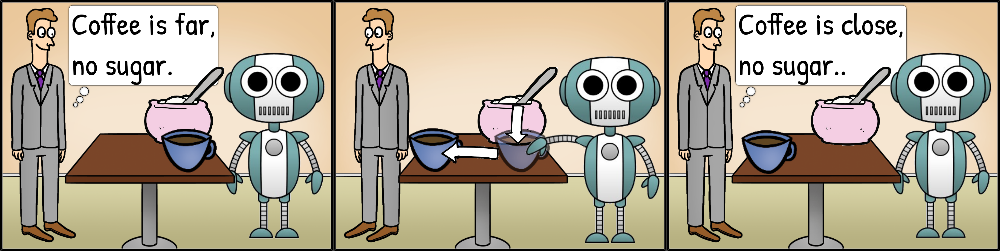
\includegraphics[width=0.9\linewidth]{figures/cartoon_inf_obs_bigger.png}
    \caption{
    % The robot adds sugar to the cup before pushing it while the human is not mindful. The position of the cup is \textit{observable}, so the human can update their belief after observing it. However, since sugar-in-cup is only \textit{inferrable}, and the human was not attentive (\textit{i.e.}, not ``co-present''), the human cannot tell whether sugar is added in the cup.
    % While  
    Human is not attentive when Robot adds sugar to the cup before pushing it forward. \textit{Assessing} the new situation after the two actions, Human can only ``know'' the cup's new position (\textit{observable}), but not \textit{SugarInCup} (\textit{inferrable}).
    }
    \label{fig:obs_attr}
\end{figure}

To better understand these observability classes, consider a scenario with a cup of coffee and some sugar on the table as depicted in Figure~\ref{fig:obs_attr}. 
Initially, the cup is far from the human and without sugar. While the human is not attentive (i.e., not \textit{co-present}, say) to the scenario, the robot adds some sugar to the cup and pushes it towards the human. 
Once the human is attentive again, they
can notice that the cup is closer. We can say that the position of the cup is \textit{observable}.
However, without observing the robot adding sugar, the human cannot know if some sugar is added to the cup. Hence, we say the \textit{SugarInCup} attribute is \textit{inferrable}, 
and the human agent would know if they observed the robot adding it. 

\subsection{Situation Assessment Modeling}

\begin{definition} \label{def:obs}
    \textbf{(Observation.)} Rblabl.  
\end{definition}

\begin{definition} \label{def:inf}
    \textbf{(Inference.)} Rblabl.  
\end{definition}

\textbf{(\textit{Action Observability}.)}
An action executed by an agent is \textit{observed} by other agents \emph{co-present} throughout the action execution. Therefore, we state that if an agent observes an action getting executed, the agent will infer the \textit{inferrable} effects of the action.
Consequently, the agent immediately updates its belief state while each inferrable attribute affected by the action receives a new value.  


\section{Belief Updates}
An agent's belief can get updated in four ways as follows. 

\subsection{Nominal Workflow}

For each action, post its execution, the workflow for updating agents' beliefs is: (1.) the acting agent's belief is updated; (2.)
for the co-present agents, their beliefs are updated based on what they \textit{infer};
and (3.) \textit{situation assessment} updates their beliefs with respective \textit{observable} facts. 
To update initial observable facts, first, a dummy action is executed with no precondition and effect.

\subsubsection{1. When Acting:}
If the agent executes an action, its belief is updated based on its effects. The state attributes appearing in the action's effect get updated with the new values, while the remaining attributes keep their same old values.

\subsubsection{2. When Inferring:}
% \hspace{-0.05in}

We do not yet consider cases where the robot's beliefs can diverge, too, assuming that, while not being observed, humans only make deterministic moves. Hence, regardless of the co-presence, the robot always updates its belief with both the \textit{inferrable} and \textit{observable} effects.

\subsubsection{3. When Observing:}
The agent assesses the situation from its current location 
with the help of spatial reasoning and its reference frame, i.e., the formalized \textit{observability} model. Consequently, the agent updates its existing belief with the relevant ground truth. 

(Based on Definition~\ref{def:pssav}) We can always associate specific state attributes to \textit{places}. 
For example, suppose that being in the state $s_1$, the robot switches on the furnace placed in \textit{kitchen}, and this generates a new state $s_2$. Also, assume that
$f_{\textit{TurnOn}}
$ is $\observable$ (Definition~\ref{def:svof}).   
Then, the \text{place specific attribute function}, $f_{loc} : (...)$, w.r.t. the states
$s_1$ and 
$s_2$ can be expressed as, 
$f_{\textit{loc}} (f_{\textit{TurnOn}}^{s_1} )$ and $f_{\textit{loc}} (f_{\textit{TurnOn}}^{s_2} )$, respectively, and both map to $\textit{kitchen} \in Places$.

Consider the following scenario: The search progresses from $s_2$, along $s_1, s_2, ...$, such that the next action applicable in it is, the agent $(\varphi_h)$ \textit{moving} to the kitchen. This generates a new state $s_3$, and hence $f_{\textit{loc}} (f_{\textit{AgtAt}}(\varphi_h, s_3) )$ maps to $kitchen$, but so does  $f_{\textit{loc}} (f_{\textit{TurnOn}}^{s_3})$. 
In such cases, $\varphi_h$ assesses the \textit{status} of the furnace, i.e., the exact value of $f_{\textit{TurnOn}}^{s_3}$ in $s_3$, which is {\sc on}, and hence the human agent updates their belief.  

Note that the robot is always aware of the ground reality hence, technically, the idea 
is effective only for the human agent. Here, the robot takes the human's perspective and performs spatial reasoning as per the human's frame of reference or their current location in the environment. 
The human's belief is updated w.r.t. what they can see as ground truth (mimicked by the robot).
This enables $\varphi_h$ to learn an \textit{observable} attribute's value achieved earlier by the robot.

The agent updates its belief with relevant ground truth learned via situation assessment, performed ``immediately'' after the execution of each action. 
Hence, the robot performs situation assessment for the human and itself.


\subsection{Handling Ambiguous Situation}

\subsubsection{Detection}

The human and robot agents carry individual, distinct belief states w.r.t. the ground truth ($s$) (s.t. $\mathit{B}_{\varphi_r}^s$ is aligned with it), while the two can be either different or aligned. 
However, the agents act as if they are certain about their knowledge.  
Since the robot plans for both, it reasons about their distinct beliefs and manages the evolution of their individual beliefs. E.g., the robot adding salt to the pasta while the human being co-present or not can grow their belief states differently. 

To produce a legal joint-plan, the robot is fine with such a divergence unless it has an \textit{adverse} effect, e.g., the human acting based on their false belief.
At a stage, if the human agent, based on $\mathit{B}_{\varphi_h}^{s_i}$, can perform a set of actions that differs from what they could perform w.r.t. to $\mathit{B}_{\varphi_r}^{s_i}$ (or the ground reality), then we say that such divergent beliefs are \textit{relevant} to be \textit{tackled}.
A divergence is also declared as \textit{relevant} if an action has different effects w.r.t. the other agent's belief.

One approach to tackle it could be to trace back to the action that creates this divergence and {\em DELAY} it for future, if and when possible. E.g., the robot delays adding salt until the human arrives in the kitchen. 
Second, communicating relevant divergences to the human agent, and it is our main focus in this work. (However, delaying may not always find a solution, but it could reduce communication requirements. Our pilot development and results are in \textit{Appendix~C}.)

Assessing the impact of different human actions (based on their wrong $\mathit{B}_{\varphi_h}^{s_i}$) or effects, with their overall positive and detrimental impacts on achieving a joint task can be interesting.
An approach can be to analyze the agents' plan history or future actions to decide whether their beliefs should get aligned or not, or for that matter, how much to communicate, but it is out of the scope of this work. 

\subsubsection{Solved by comm minimally}

Its belief gets updated by learning ground truth when another agent communicates an attribute-value pair. Communication occurs via a \textit{distinct set} of actions, modeled as a predefined communication protocol for a pair of sender-receiver agents. 

As the robot is always aware of ground truth, again, technically, it is effective only for the human belief.
We note that each action communicates only {\em one} attribute-value pair, so just one attribute gets updated in the human belief.

We establish protocols between each \textit{sender-receiver} agents pair for communication, 
and model explicit communication actions between them. 
Note that these actions are different than agents' (non-) primitive actions.

\subsection{Modeling Communication Actions} 
Suppose there exists a state-variable function, $f_{svs}:(?g_1 (gr_1), ?g_2 (gr_2), ..., ?g_k (gr_k),\mathcal{S}) \rightarrow ?g_{k+1} (gr_{k+1})$ such that,
for the current world state $s \in \mathcal{S}$, the corresponding state attribute, $f_{\textit{svs}}(g_{(1)l},g_{(2)m},...,g_{(k)n},s)$ maps to $q$.

An agent $\varphi_i$ can communicate this attribute-value pair to another agent $\varphi_j$, if the following conditions meet as action precondition: 
(1.) For $\varphi_i$, its belief state satisfies the fact being communicated, i.e.,
$f_{\textit{svs}}(g_{(1)l},g_{(2)m},...,g_{(k)n},B_{\varphi_i}^s) = q$, and (2.) $\varphi_j$'s belief state does not satisfy this truth, i.e., $f_{\textit{svs}}(g_{(1)l},g_{(2)m},...,g_{(k)n},B_{\varphi_j}^s) = r$ such that $r \neq q$.
The effect of this action is that now 
$\varphi_j$'s belief is updated, i.e., $f_{\textit{svs}}(g_{(1)l},g_{(2)m},...,g_{(k)n},B_{\varphi_j}^s) \leftarrow q$. 

At this stage, say, the ground truth ($s_i$), we assume \textit{Updates Workflow} was already called, and then the sender reasoned out and decided to \textit{tackle} the receiver's divergent beliefs. 

\subsubsection{Communicate Only The Required Facts.}
Note that there exists at least one \textit{attribute}-\textit{value} in receiver's belief state causing adverse effects. 
The approach, explained in the next \textit{three} steps, looks for the minimal number of such attribute-value pairs to be communicated so that
the divergence in the updated belief is made \textit{irrelevant}, or even eliminated.
\begin{enumerate}
    \item 
    \textit{Store} each attribute and its value if the attribute's value differs in the receiver's belief from the sender's belief. 

    \item For them, \textit{build} actions, $\textit{comm-action}_i$, following the schema described earlier. Say, they are equally costly.  
    
    \item 
    (Follow Breadth-First Search) 
    The \textit{source} is $B_{\varphi_h}^{s_i}$, and each $\textit{comm-action}_i$ changes and aligns \textit{exactly} one attribute while its updated value satisfies the ground truth. If $\textit{comm-action}_i$ is applied, generates a new belief state (following the regular state transition rules), using: $B_{\varphi_h}^{s_i,1} = \gamma(B_{\varphi_h}^{s_i}, \textit{comm-action}_i)$.
    It continues until the first (updated) belief is selected to expand s.t. its remaining divergence is \textit{ineffective}. We then \textit{retrieve} all the actions used from the root until the current belief state.   
\end{enumerate}

These retrieved actions are appended to the sender's plan.

\subsubsection{Solved by delaying RA}

%%%%%%%%%%%%%%%%%%%%%%%%%%%%%%%%%%%%%%%%%%%%%%%%%%%%%%%%%%%%%%%%%%%%%%%%%



\section{Formal Properties}
Note that our solver has a similar high-level elaboration process, i.e., its underlying mechanism, as the old solver but with a better estimation of the evolution of agents' beliefs.  
However, when discussing its soundness and completeness, dependent on the soundness and completeness of the underlying mechanism, we must distinguish between the problem specifications used by these solvers. 

In the worst-case, our specifications would pick each $p \in P$ (all propositions), generate a new set of primitive propositions for every possible combinations of $|\{\observable,\inferrable\}| \times |\mathit{Places}|$. 
So, the size of the new encoding for primitive propositions is worst-case \textit{linear} in the size of $P$.

For the old specifications and to support the old solver's simplified assumptions, an equivalent encoding to the above can be considered $p$ belonging to the $\inferrable$ class for every $place \in \mathit{Places}$, and the agents can \textit{always} be considered co-present.  
Note that for a domain like Blocksworld where explicit modeling of $\mathit{Places}$ is not required, it considers a \textit{single} dummy place $p_{du}$ (depicting that everything occurs here) to serve this new encoding. So, it \textit{ensures} that transformed formalism captures everything that can be formulated using the original dual-HTNs but technically provides a latitude to model more realistic problems. 

\begin{theorem}
\textbf{(Soundness.)} The new solver is sound.
\vspace{-0.06in}
\begin{proof}
Following Definition~\ref{def:joint-sol-plan},
we show that the joint solution plan generated is executable:
For a branch, it is guaranteed that it meets the {\em solution conditions}.
Moreover, each precondition for an agent's action is achieved in earlier time stamps by either: its own action, 
\textit{inferred} while observing another agent's actions, 
another agent \textit{communicated},
or it is \textit{assessed} by observing a situation and reasoning.
Of course, another agent’s action supplying the precondition, an attribute (in $\observable$) and its value, cannot be destroyed. 
Hence this branch/trace is executable.

Finally, since the human can make any choices during execution,
and are unknown upfront, any of its branches, by the
above argument, will be executed. 
Implies, the joint solution plan is executable.
\end{proof}
\end{theorem}

\begin{theorem}
\textbf{(Completeness.)} The new planning algorithm is complete, provided the underlying mechanism can exhaustively generate all possible plan elaborations. 
\vspace{-0.06in}
\begin{proof}
Suppose a problem modeled based on our formalism has a solution, say, a joint solution tree, $\tau$ and is sound. 
From $\tau$, remove all the communication and situation assessment steps, and say it generates $\tau'$. Now, relax the original problem, considering all the agents being always co-present and making all the propositions \textit{inferrable} everywhere. 
Technically, the solver will generate $\tau'$ for this new problem when it exhaustively generates the whole search space (of course, it may contain redundant actions). 
We assure it believing on the underlying mechanism and that there is at least one solution ($\tau$) for the original problem. As a result, it is trivial to visualize that $\tau'$ is always extendable to generate $\tau$ w.r.t. the original problem. (\textit{Updates Workflow}.) After the execution of each step, one can employ the situation assessment and action's effect inference subroutines, checking for belief divergences and using communication actions if needed. 
\end{proof}
\end{theorem}

\begin{figure}[t!]
    \centering
    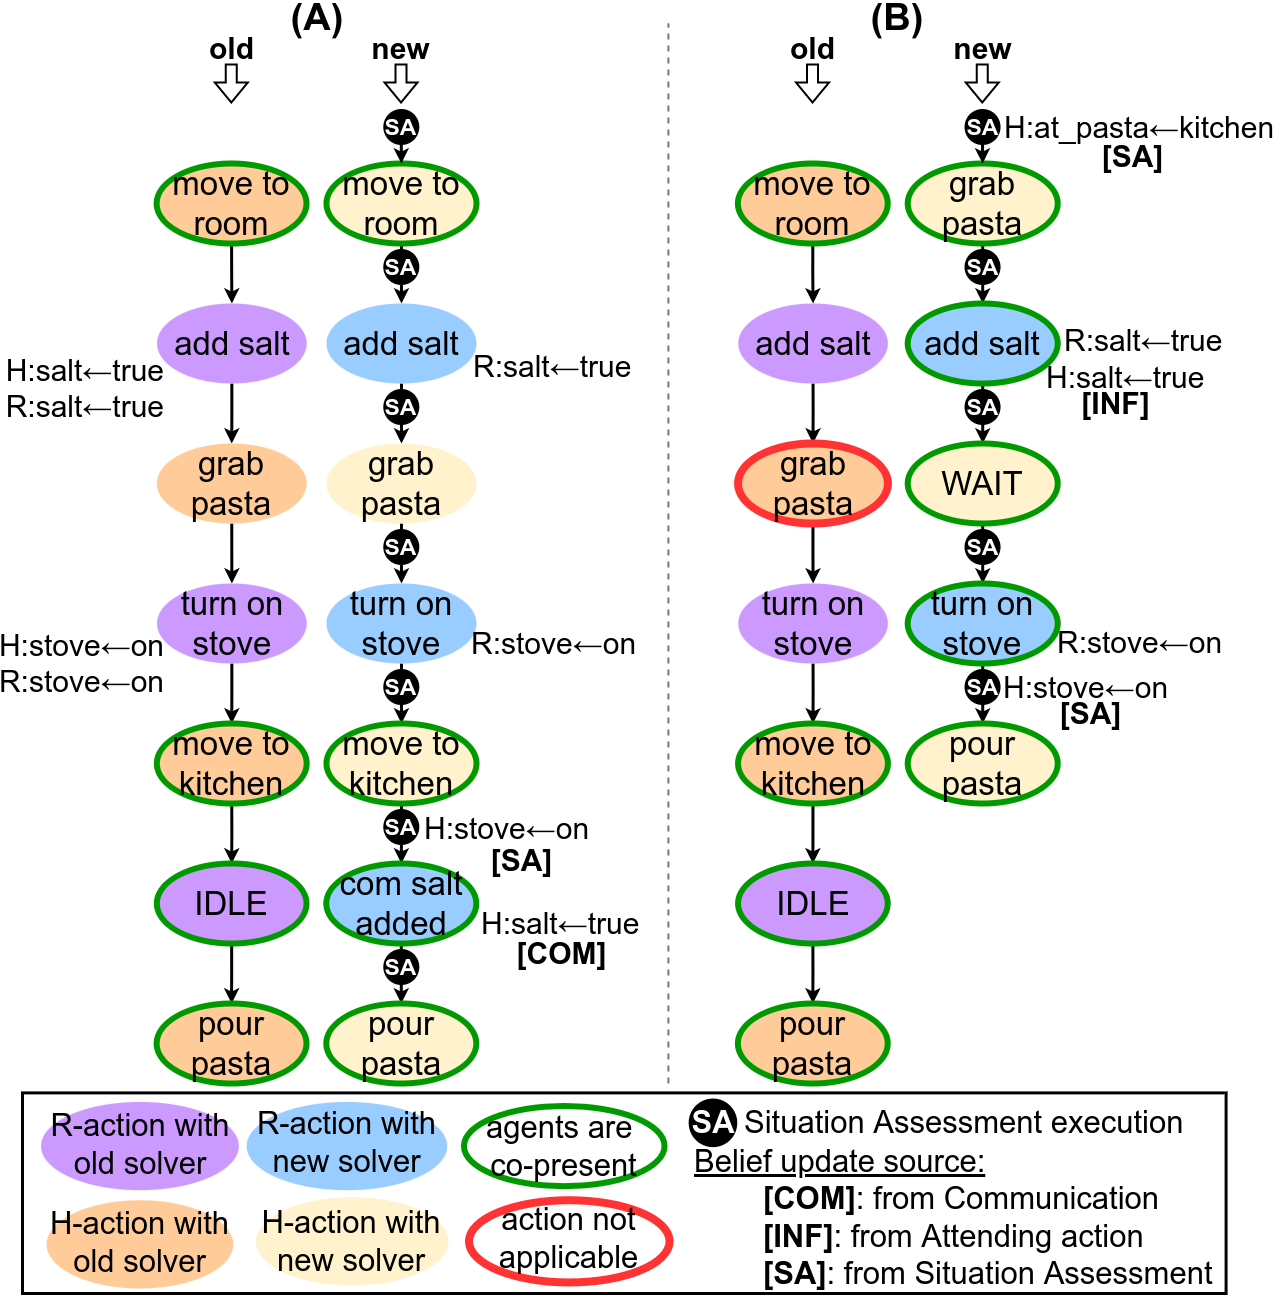
\includegraphics[width=0.99\linewidth]{figures/bc_plans.png}
    % \includegraphics[width=0.85\linewidth]{figures/new_plans.png}
    \caption{
    Plans obtained in two scenarios: Each presents two plans. (\textit{Left}) Obtained by the old solver, and (\textit{Right}) obtained by ours. The latter depicts more realistic and appropriate belief updates (focusing on two attributes).
    Case~(A): the human has no certainty on {\em SaltInPot}, while ours decides to communicate to remove the ambiguity. 
    And, Case~(B): an initial belief divergence on {\em AtPasta} induces an ``invalid'' plan, but ours predicts that the human \textit{assess} the pasta location and update their belief, without being communicated.
    }
    \label{fig:scenarios}
\end{figure}

    

\section{Evaluation}

Before we describe three {\em novel} domains used in the experiments and the results to compare the old and new approaches, let us make a ``high-level'' distinction between the two. 
In principle, the old solver can handle a belief divergence only when agents start with unaligned, distinct beliefs. But, when it is not so, unlike ours, it assumes that the agents' beliefs never diverge during planning, and hence there is no way it can handle a divergence created by an agent in practice. 
The old solver can align the beliefs via explicitly influencing (the human's) action model and a cumbersome technique using triggers to update their task networks. Our approach estimates the evolution of belief divergences at planning time and uses explicit communication actions to handle them in practice to generate robust plans. 

\subsubsection{Cooking Pasta Domain:}
Suppose a stove and salt are available in \textit{Kitchen} $\in$ $\textit{Places}$, and the pasta can be either in \textit{Kitchen} or \textit{Room} (the two are adjacent). The agents have different roles and can only operate in the two places. Robot \textit{adds} salt to the pot and \textit{turns-on} the stove. Human \textit{grabs} the pasta and \textit{pours} it into the pot. 
Pasta can be poured after salt is added to the pot and the stove is {\sc on}.
Focus on the following two attributes associated to \textit{Kitchen}: For a given state, $s_i \in \mathcal{S}$, $f_{\textit{SaltInPot}}^{s_i} \in \{\textit{true, false}\}$ and $f_{\textit{stove}}^{s_i} \in \{\textit{on, off}\}$ such that only $f_{\textit{stove}}^{s_i}$ is \textit{inferrable}, all others belong to $\observable$.

\subsubsection{Preparing Box Domain:}
A box filled with a fixed number of balls with a sticker on it is considered prepared and needs to be sent. Both the agents can \textit{fill} the box with balls from a bucket, while only the robot can \textit{paste} a sticker and only the human can \textit{send} the box. The bucket can run out of balls, so when only one ball is left, the human \textit{moves} to another room to \textit{grab} more balls and \textit{refill} it. 
The number of balls in the box is \textit{inferrable}, while all other variables are {\em observable}. 

\subsubsection{Car Maintenance Domain:}
The washer fluid ($\observable$) and engine oil ($\inferrable$) levels have to be \textit{full} before \textit{storing} the oil gallon in the cabinet ($\inferrable$). 
Only the robot can \textit{refill} both the tanks and store the gallon while situated at \textit{Front} of the car. 
\textit{Front-left} and \textit{Front-right} headlights have to be \textit{checked} and a light-bulb has to be \textit{replaced} at \textit{Rear}. 
Only the human can check and replace lights, and they can start with either of these two tasks.
Both agents starts at \textit{Front}.
The car's hood needs to be \textit{closed} by the human at last.

\subsection{Qualitative Analysis}

In the first domain, we highlight \textit{subtleties} the old solver overlooks and how ours is aware of them, updates beliefs, and effectively manages divergences. 
We discuss the plans obtained in two scenarios 
as shown in Figure~\ref{fig:scenarios}. Assume that both the agents are in \textit{Kitchen} and the human acts first. Scenario~(A): Captures the agents' plans when the pasta is in \textit{Room}. 
Scenario~(B): 
In hindsight, the pasta is moved from \textit{Room} to {\em Kitchen}, which the robot knows, while the human still has the old belief.

\begin{itemize}
    % \item \textbf{Scenario~(A):} 
    % Although the solvers generate similar plans, they update the human's belief differently if and when the human and robot are co-present. E.g., turning on the stove ideally (realistically) does not affect the human's mental state, which is not the case for the old solver. It considers agents omniscient, so the human knows everything immediately once achieved. 
    % Our solver predicts it when the human returns to the kitchen and assesses that the stove is {\sc on}, and their belief gets updated.
    \item \textbf{Scenario~(A):} 
    % The human leaves the kitchen and hence practically is unaware of the changes achieved in the environment by the robot's actions: {\em turn on} and {\em add salt}. 
    As the human left {\em Kitchen}, practically, they are unaware of the changes caused by the robot's actions: {\em turn on} and {\em add salt}. (\textit{Left}) The old solver considers agents omniscient. So, the human knows that the stove is {\sc on}, and salt is added even before arriving back in {\em Kitchen}. (\textit{Right}) Thanks to both situation assessment and inference based on action observability, it estimates that when returning to the kitchen, the human assesses that the stove is {\sc on}. Moreover, it predicts that the human cannot know \textit{SaltInPot} and that this divergence, identified as relevant, needs to be handled via communication.
    % The old solver considers agents omniscient, i.e., they know everything immediately once achieved. Hence, the human knows that the stove is {\sc on}, and salt is added even before being back in \textit{Kitchen}.
    % The new solver, thanks to both an appropriate situation assessment and inference based on action observability, estimates that when returning to the kitchen, the human assesses that the stove is {\sc on}.
    % Moreover, it predicts that the human cannot know the \textit{SaltInPot} fact and that this divergence, identified as relevant, needs to be handled via communication. 
    % This divergence was ineffective after the robot communicates it to the human.
    \item
    % \textbf{Scenario~(C):} In the updated scenario, using the old approach, the human moves to \textit{Room} to grab the pasta, but in reality, the action \textit{fails} as it is not a legal action w.r.t. the robot's belief or the ground truth. But, the way our planning system works, the human agent assesses the
    \textbf{Scenario~(B):}
    % With the old solver, 
    (\textit{Left}) the human moves to \textit{Room} to \textit{grab} the pasta, but in reality, being an illegal action w.r.t. 
    % the robot's belief or 
    the ground truth, it \textit{fails}. 
    (\textit{Right}) the human agent \textit{assesses} the environment to update their beliefs, knowing \textit{PastaInKitchen}. 
    % Also, no communication is required for this update. 
    Hence, no communication is required.
    % environment and updates their belief state, knowing that the pasta is in the kitchen. Hence no communication is required to align their belief. The rest is self-evident.
\end{itemize}

\begin{table}
    \begin{adjustbox}{width=0.77\columnwidth,center}
    \begin{tabular}{@{}c|r r r| c@{}}
        % \hline
        \multirow{2}{*}{
        \textbf{Domain}} & \multicolumn{3}{c|}{\textbf{\textit{Old Solver}}} & \multicolumn{1}{c}{\textbf{\textit{Our Solver}}}
        \\
        % \cline{2-6}
        & \multicolumn{1}{c}{\textit{S}} & \multicolumn{1}{c}{\textit{NA}} & \multicolumn{1}{c|}{\textit{IDL}} & \multicolumn{1}{c}{\textit{Com}} 
        \\ \cline{1-5}
        \textit{Cooking} & 18.6\% & 77.0\% & 23.0\%  & 54.9\%\\
        \textit{Box} & 25.0\% & 83.3\% & 16.7\%  & 68.8\%\\
        \textit{Car} & 12.5\% & 73.2\% & 26.8\%  & 79.7\%\\
        \hline
        \textbf{Average} & 18.7\% & 77.8\% & 22.2\%  & 67.8\%\\
    \end{tabular}
    \end{adjustbox}
    \caption
    {
    \label{tab:q_results}
    % Comparison of the two solvers on the two domains. 
    % In each domain: 
    For the \textit{old solver}, the success rate (\textit{S}), the ratio of failed plans due to a non-applicable action (\textit{NA}), and the ratio of failed plans due to an inactivity deadlock case (\textit{IDL}), while for \textit{our solver}: (the success rate is always 100\%), the ratio of plans including a communication action (\textit{Com}).
    }
\end{table}

\subsection{Experimental results}

Quantitative results in three new domains appear in Table~\ref{tab:q_results}. 
We consider (in box domain) \textit{three} boxes to be prepared and sent. 
In each domain, we generated 512 different initial states, including 448 (87.5\%) with divergent initial beliefs and 64 states where beliefs are fully aligned initially. 
Overall, 3072 plans were generated.

With the old approach, a planning failure occurs due to: 
(a) an action of a plan not applicable in another agent's belief state, including the ground truth; 
(b) if an inactivity deadlock occurs, which is assumed to be the case after a succession of at least four {\em WAIT} and (or) {\em IDLE} actions. 
Such deadlocks occur when the human has a belief divergence and waits for a never-happening robot's action, e.g., waiting for \textit{adding} salt, but \textit{SaltInPot} is already achieved.
For the old solver, the success rate (\textit{S}), the \textit{ratios} of the number of failed plans due to a inapplicable action (\textit{NA}) and to an inactivity deadlock (\textit{IDL}) appear in the table.
For ours, the \textit{ratio} of successful plans with a communication action is presented under \textit{Com}.

As the old solver does not handle belief divergence in planning, the applicability of actions is never an issue w.r.t. another agent's beliefs. 
Therefore, if the \textit{IDL} case occurs, it is understood that the initial belief divergences are not tackled by modeling triggers explicitly in the task specifications. 

Our solver always finds legal plans, and on average $\approx$ 68\% of them use \textit{communication}.
Moreover, the robot doesn't need to communicate systematically as assessing situations handles a major part of the divergences (87.5\% of the scenarios have divergent beliefs initially).
For the old solver, if no initial belief divergence exists, it always finds a legal plan, considering the agents omniscient. 
E.g., Fig.~\ref{fig:scenarios}(A). However, sometimes, this causes problems in practice.
Scenarios beginning with unaligned beliefs induce actions often not applicable in another agent's belief state (or the ground truth), evident by the (average) 18.7\% success rate.

We can see that our solver uses more communication actions in the car maintenance domain than in the other two.
But looking at the \textit{low} old solver's success rate (12.5\%), we conclude that this domain generally needs more communication. 
Compared to others, it purposely creates non-relevant belief divergence, e.g., the robot storing the gallon in the cabinet ($\inferrable$) is irrelevant.
After a close analysis, we found that $\approx$ 42\% of the plans have divergent human beliefs at least in one branch after the last action (\textit{leaf}) was executed (i.e., \textit{irrelevant} divergences never got communicated). 

\section{Discussion}
We formalize execution-time observability conventions based on situation assessment and action observability (ToM). We use it to estimate the evolution of the human mental state and capture belief divergences. 
A new planner is described, which utilizes this better estimation of human mental state to plan for more robust and consistent human-robot joint activities such that a relevant belief divergence is tackled by explicitly modeled communication actions.  

Moreover, our effort was to make our main \textit{contributions} (i.e., formalizing observability based conventions) to have a ``generic'' description. Hence, they are not limited to only our intended framework (HATP/EHDA).

Handling these conventions formally is vital for robust planning, as otherwise, it can lead to problems at run-time. 
E.g., Fig.~\ref{fig:scenarios}(A): the human knowing \textit{SaltInPot} is ambiguous. 
Explicit reasoning on the human mental state detects ambiguous situations and removes them via communication. 

Our formalism does not refute something believed by an agent through situation assessment. 
E.g., for some $s_i \in \mathcal{S}$, if the human \textit{wrongly} believes that the pasta is in \textit{Kitchen}. The situation assessment does not help refute this, while the human is in \textit{Kitchen}. 
The reason is that $f_{\textit{PastaNotInKitchen}}^{s_i}(...)$ is not modeled explicitly as an attribute. 
And hence such issues do not affect the completeness. 
Moreover, our solver handles them as a \textit{relevant} divergence to be aligned. Followed by the human is communicated with correct updates.

\bibliography{bib.bib}

\end{document}


